\include{preamble}

\title{Procedural Terrain Generation}
\subtitle{Generating a beautiful world at runtime}
\author{\large Brothers of Destruction \\
2005041 Md Imtiaz Kabir \and \\
2005070 Md Irtiaz Kabir}
\institute{Department of Computer Science and Engineering\\ Bangladesh University of Engineering and Technology (BUET)}

\begin{document}

\begin{frame}
  \titlepage
\end{frame}

\begin{frame}{Index}
  \vspace{0.5cm}
  \tableofcontents
\end{frame}

\section{How does an endless scroller become endless?}

\begin{frame}{Why Learn This?}
    \pause
    \begin{minipage}{0.45\textwidth}
        \centering
        \includegraphics[width=\linewidth]{images/minecraft.png}
        \captionof*{figure}{3D Voxel terrain in Minecraft}
    \end{minipage}%
    \hfill
    \pause
    \begin{minipage}{0.45\textwidth}
        \centering
        \includegraphics[width=\linewidth]{images/terraria.png}
        \captionof*{figure}{2D terrain of Terraria}
    \end{minipage}

    \begin{itemize}
        \item<3-> How do your favourite games create these \textbf{beautiful} endless terrains?
        \item<4-> Create a single terrain by hand and store it somewhere, repeat when it ends.
        \item<5-> Have a set of terrains and choose one at random at start.
        \item<6-> How do we ensure nothing repeats without having infinite memory and infinite time?
        \item<7-> Analytic terrains ($y = sin(x)$) are boring and not realistic
        \item<8-> We need to somehow accommodate the randomness of nature.
    \end{itemize}
\end{frame}

\section{Generation Algorithms}


\begin{frame}{Cellullar automata}
    \begin{columns}
        \begin{column}{0.6\textwidth}
            \begin{mathbox}{Steps of algorithm}
                \only<1>{
                    \textbf{Step 1:} Start with random grid with $1$ as wall and $0$ as passage.

                }
                \only<2>{
                    \textbf{Step 2:} Each next iteration, change a cells value according to the following rule. \\
                    A cell becomes a wall, if in it's Moore neighborhood (including itself), majority of cell is wall. \\
                    Otherwise it becomes a passage.
                }
            \end{mathbox}
        \end{column}
            \begin{column}{0.4\textwidth}
      \begin{tikzpicture}[scale=0.6,
          wall/.style={fill=black, draw=gray},
          passage/.style={fill=white, draw=gray},
          highlight/.style={fill=red!30, draw=red, thick}]

          % Step 1: Random initial grid
          \only<1>{
              % Define a 6x6 random grid pattern
              \foreach \x in {0,1,2,3,4,5} {
                  \foreach \y in {0,1,2,3,4,5} {
                      \pgfmathparse{int(random(2))}
                      \ifnum\pgfmathresult=1
                          \draw[wall] (\x,\y) rectangle (\x+1,\y+1);
                          \node at (\x+0.5,\y+0.5) {\tiny 1};
                      \else
                          \draw[passage] (\x,\y) rectangle (\x+1,\y+1);
                          \node at (\x+0.5,\y+0.5) {\tiny 0};
                      \fi
                  }
              }
              \node[below] at (3,-0.5) {Random Initial Grid};
          }

          % Step 2: Show Moore neighborhood rule
          \only<2>{
              % Fixed pattern to demonstrate the rule
              % Grid with specific pattern
              \draw[passage] (0,0) rectangle (1,1); \node at (0.5,0.5) {\tiny 0};
              \draw[wall] (1,0) rectangle (2,1); \node at (1.5,0.5) {\tiny 1};
              \draw[passage] (2,0) rectangle (3,1); \node at (2.5,0.5) {\tiny 0};
              \draw[wall] (3,0) rectangle (4,1); \node at (3.5,0.5) {\tiny 1};
              \draw[passage] (4,0) rectangle (5,1); \node at (4.5,0.5) {\tiny 0};
              \draw[wall] (5,0) rectangle (6,1); \node at (5.5,0.5) {\tiny 1};

              \draw[wall] (0,1) rectangle (1,2); \node at (0.5,1.5) {\tiny 1};
              \draw[wall] (1,1) rectangle (2,2); \node at (1.5,1.5) {\tiny 1};
              \draw[highlight] (2,1) rectangle (3,2); \node at (2.5,1.5) {\tiny ?};
              \draw[wall] (3,1) rectangle (4,2); \node at (3.5,1.5) {\tiny 1};
              \draw[passage] (4,1) rectangle (5,2); \node at (4.5,1.5) {\tiny 0};
              \draw[passage] (5,1) rectangle (6,2); \node at (5.5,1.5) {\tiny 0};

              \draw[passage] (0,2) rectangle (1,3); \node at (0.5,2.5) {\tiny 0};
              \draw[wall] (1,2) rectangle (2,3); \node at (1.5,2.5) {\tiny 1};
              \draw[wall] (2,2) rectangle (3,3); \node at (2.5,2.5) {\tiny 1};
              \draw[passage] (3,2) rectangle (4,3); \node at (3.5,2.5) {\tiny 0};
              \draw[wall] (4,2) rectangle (5,3); \node at (4.5,2.5) {\tiny 1};
              \draw[passage] (5,2) rectangle (6,3); \node at (5.5,2.5) {\tiny 0};

              % Continue pattern for remaining rows
              \draw[wall] (0,3) rectangle (1,4); \node at (0.5,3.5) {\tiny 1};
              \draw[passage] (1,3) rectangle (2,4); \node at (1.5,3.5) {\tiny 0};
              \draw[wall] (2,3) rectangle (3,4); \node at (2.5,3.5) {\tiny 1};
              \draw[wall] (3,3) rectangle (4,4); \node at (3.5,3.5) {\tiny 1};
              \draw[passage] (4,3) rectangle (5,4); \node at (4.5,3.5) {\tiny 0};
              \draw[wall] (5,3) rectangle (6,4); \node at (5.5,3.5) {\tiny 1};

              % Highlight Moore neighborhood around center cell
              \draw[red, thick, dashed] (1.5,0.5) rectangle (3.5,2.5);
              
              \node[below] at (3,-0.5) {Moore Neighborhood Rule};
          }
      \end{tikzpicture}
  \end{column}


    \end{columns}
    
\end{frame}

\begin{frame}{Cellullar automata: Demonstration}
    \pause
    \includegraphics[height=7cm]{images/ca.png}
\end{frame}

\begin{frame}{Midpoint Displacement Algorithm}
    \begin{columns}
        \begin{column}{0.6\textwidth}
            \begin{mathbox}{Steps of algorithm}
                \only<1>{
                    \textbf{Step 1:} Begin with a straight line segment $AB$.

                }
                \only<2>{
                    \textbf{Step 2:} Compute the midpoint $C$ of $AB$
                    \begin{align*}
                        C = \frac{A+B}{2}
                    \end{align*}
                }
                \only<3>{
                    \textbf{Step 3:} Compute unit normal $\hat{n}$ of segment $AB$ 
                    \begin{align*}
                        \hat{n} = \frac{B - A}{|B-A|} \times \hat{k}
                    \end{align*}
                }
                \only<4>{
                    \textbf{Step 4:} Multiply with \texttt{random(-h, h)} to find displacement \vec{s}
                    \begin{align*}
                        \vec{s} = \hat{n} \times \texttt{random(-h, h)}
                    \end{align*}
                }

                \only<5>{
                    \textbf{Step 5:} Displace midpoint
                    \begin{align*}
                        C' = C + \vec{s}
                    \end{align*}
                }
                
                \only<6>{
                    \textbf{Step 6:} Remove old line segment ($AB$) and add new segments ($AC', BC'$)
                }
                
                \only<7->{
                    \textbf{Step 7:} Repeat the process (with geometrically reduced $h$) $n$ times to create a terrain with $2^n + 1$ points
                }
            \end{mathbox}
        \end{column}
              \begin{column}{0.4\textwidth}
          \begin{tikzpicture}[scale=1.2]
              % Define coordinates
              \coordinate (A) at (0, 1);
              \coordinate (B) at (3, 1);
              \coordinate (C) at (1.5, 1);
              \coordinate (Cp) at (1.5, 3);

              % Step 1: Initial line segment
              \only<1>{
                  \draw[thick, ObjectColor] (A) -- (B);
                  \fill[ObjectColor] (A) circle (1.5pt) node[below left] {$A$};
                  \fill[ObjectColor] (B) circle (1.5pt) node[below right] {$B$};
              }

              % Step 2: Show midpoint
              \only<2>{
                  \draw[thick, ObjectColor] (A) -- (B);
                  \fill[ObjectColor] (A) circle (1.5pt) node[below left] {$A$};
                  \fill[ObjectColor] (B) circle (1.5pt) node[below right] {$B$};
                  \fill[PrimaryColor] (C) circle (1.5pt) node[below] {$C$};
                  \draw[dashed, gray] (C) -- (1.5, 0.5);
              }

              % Step 3: Show normal vector
              \only<3>{
                  \draw[thick, ObjectColor] (A) -- (B);
                  \fill[ObjectColor] (A) circle (1.5pt) node[below left] {$A$};
                  \fill[ObjectColor] (B) circle (1.5pt) node[below right] {$B$};
                  \fill[PrimaryColor] (C) circle (1.5pt) node[below] {$C$};
                  \draw[->, AccentColor, thick] (C) -- (1.5, 2) node[right] {$\hat{n}$};
              }

              % Step 4: Show displacement vector
              \only<4>{
                  \draw[thick, ObjectColor] (A) -- (B);
                  \fill[ObjectColor] (A) circle (1.5pt) node[below left] {$A$};
                  \fill[ObjectColor] (B) circle (1.5pt) node[below right] {$B$};
                  \fill[PrimaryColor] (C) circle (1.5pt) node[below] {$C$};
                  \draw[->, red, thick] (C) -- (Cp) node[midway, right] {$\vec{s}$};
              }

              % Step 5: Show displaced midpoint
              \only<5>{
                  \draw[thick, ObjectColor] (A) -- (B);
                  \fill[ObjectColor] (A) circle (1.5pt) node[below left] {$A$};
                  \fill[ObjectColor] (B) circle (1.5pt) node[below right] {$B$};
                  \fill[gray!50] (C) circle (1.5pt);
                  \fill[SecondaryColor] (Cp) circle (1.5pt) node[above] {$C'$};
                  \draw[dashed, gray] (C) -- (Cp);
              }

              % Step 6: Show new line segments
              \only<6>{
                  \draw[thick, PrimaryColor] (A) -- (Cp);
                  \draw[thick, PrimaryColor] (Cp) -- (B);
                  \fill[ObjectColor] (A) circle (1.5pt) node[below left] {$A$};
                  \fill[ObjectColor] (B) circle (1.5pt) node[below right] {$B$};
                  \fill[SecondaryColor] (Cp) circle (1.5pt) node[above] {$C'$};
              }

              % Step 7: Show further iterations
              \only<7->{
                  % First iteration result
                  \draw[dashed, thick, PrimaryColor] (A) -- (Cp) -- (B);

                  % Second iteration points
                  \coordinate (M1) at (1, 1.5);
                  \coordinate (M2) at (3, 1.8);

                  \draw[thick, AccentColor] (A) -- (M1) -- (Cp) -- (M2) -- (B);

                  \fill[ObjectColor] (A) circle (1pt) node[below left, scale=0.8] {$A$};
                  \fill[ObjectColor] (B) circle (1pt) node[below right, scale=0.8] {$B$};
                  \fill[SecondaryColor] (Cp) circle (1pt);
                  \fill[AccentColor] (M1) circle (1pt);
                  \fill[AccentColor] (M2) circle (1pt);

                  \node[below, scale=0.8] at (2, 0.3) {Terrain after 2 iterations};
              }
          \end{tikzpicture}
      \end{column}

    \end{columns}
    \only<8->{
        \begin{conceptbox}{Making it endless}
            \begin{itemize}
                \item \textbf{Two terrains} Create two overlapping terrains
                \item \textbf{Swap and create} When the first terrain goes out of screen swap the terrains and replace the later terrain with a new one.
            \end{itemize}
        \end{conceptbox}
    }
\end{frame}

\begin{frame}{Midpoint Displacement Algorithm: Demonstration}
    \pause
    \includegraphics[height=7cm]{images/2d-terrain.png}
\end{frame}


\begin{frame}{Terrain with Perlin Noise}
    \begin{columns}
        \begin{column}{0.6\textwidth}
            \begin{mathbox}{Steps of algorithm}
                \only<1>{
                    \textbf{Step 1:} Begin with a tessellation of a region in $xy$ plane. \\
                    Store the tessellation as a list of lattice points.

                }
                \only<2>{
                    \textbf{Step 2:} For each lattice points use Perlin noise to compute the terrain height.
                    \begin{align*}
                        h(x,y) = \texttt{height} \times \texttt{perlin(x,y)}
                    \end{align*}
                }
                \only<3->{
                    \textbf{Step 3:} Extrude each lattice point in tessellation 
                    \begin{align*}
                        C' = C + h(x,y) \times \hat{k}
                    \end{align*}
                }
            \end{mathbox}
        \end{column}
          \begin{column}{0.4\textwidth}
      \begin{tikzpicture}[scale=0.8,
          x={(1cm,0cm)}, y={(0.5cm,0.5cm)}, z={(0cm,1cm)},
          point/.style={circle, fill, inner sep=1.5pt}]

          % Step 1: Connected 4x4 grid of lattice points
          \only<1>{
              % Draw grid connections
              \foreach \x in {0,1,2,3} {
                  \draw[ObjectColor, thick] (\x,0,0) -- (\x,3,0);
              }
              \foreach \y in {0,1,2,3} {
                  \draw[ObjectColor, thick] (0,\y,0) -- (3,\y,0);
              }
              % Draw lattice points
              \foreach \x in {0,1,2,3} {
                  \foreach \y in {0,1,2,3} {
                      \node[point, ObjectColor] at (\x,\y,0) {};
                  }
              }
              \node[below] at (1.5,-0.5,0) {Connected Grid};
          }

          % Step 2: Show height calculation on one point
          \only<2>{
              % Draw base grid
              \foreach \x in {0,1,2,3} {
                  \draw[ObjectColor, thick] (\x,0,0) -- (\x,3,0);
              }
              \foreach \y in {0,1,2,3} {
                  \draw[ObjectColor, thick] (0,\y,0) -- (3,\y,0);
              }
              % Draw all base points
              \foreach \x in {0,1,2,3} {
                  \foreach \y in {0,1,2,3} {
                      \node[point, ObjectColor] at (\x,\y,0) {};
                  }
              }
              % Show height calculation for center point
              \draw[dashed, PrimaryColor, thick] (1,1,0) -- (1,1,1.5);
              \node[point, PrimaryColor] at (1,1,1.5) {};
              \node[right, PrimaryColor] at (1,1,0.75) {h(x,y)};
          }

          % Step 3: Extrude all points with connections
          \only<3->{
              % Define height function (simple for visualization)
              \pgfmathsetmacro{\ha}{0.3}
              \pgfmathsetmacro{\hb}{0.8}
              \pgfmathsetmacro{\hc}{1.2}
              \pgfmathsetmacro{\hd}{0.6}

              % Draw extruded grid connections
              \draw[ObjectColor, thick] (0,0,\ha) -- (1,0,\hb) -- (2,0,\hc) -- (3,0,\hd);
              \draw[ObjectColor, thick] (0,1,\hb) -- (1,1,\hc) -- (2,1,\hd) -- (3,1,\ha);
              \draw[ObjectColor, thick] (0,2,\hc) -- (1,2,\hd) -- (2,2,\ha) -- (3,2,\hb);
              \draw[ObjectColor, thick] (0,3,\hd) -- (1,3,\ha) -- (2,3,\hb) -- (3,3,\hc);

              \draw[ObjectColor, thick] (0,0,\ha) -- (0,1,\hb) -- (0,2,\hc) -- (0,3,\hd);
              \draw[ObjectColor, thick] (1,0,\hb) -- (1,1,\hc) -- (1,2,\hd) -- (1,3,\ha);
              \draw[ObjectColor, thick] (2,0,\hc) -- (2,1,\hd) -- (2,2,\ha) -- (2,3,\hb);
              \draw[ObjectColor, thick] (3,0,\hd) -- (3,1,\ha) -- (3,2,\hb) -- (3,3,\hc);

              % Draw extruded points
              \node[point, AccentColor] at (0,0,\ha) {};
              \node[point, AccentColor] at (1,0,\hb) {};
              \node[point, AccentColor] at (2,0,\hc) {};
              \node[point, AccentColor] at (3,0,\hd) {};
              \node[point, AccentColor] at (0,1,\hb) {};
              \node[point, AccentColor] at (1,1,\hc) {};
              \node[point, AccentColor] at (2,1,\hd) {};
              \node[point, AccentColor] at (3,1,\ha) {};
              \node[point, AccentColor] at (0,2,\hc) {};
              \node[point, AccentColor] at (1,2,\hd) {};
              \node[point, AccentColor] at (2,2,\ha) {};
              \node[point, AccentColor] at (3,2,\hb) {};
              \node[point, AccentColor] at (0,3,\hd) {};
              \node[point, AccentColor] at (1,3,\ha) {};
              \node[point, AccentColor] at (2,3,\hb) {};
              \node[point, AccentColor] at (3,3,\hc) {};

              \node[below] at (1.5,-0.5,0) {3D Terrain};
          }
      \end{tikzpicture}
  \end{column}


    \end{columns}
    \only<4->{
        \begin{conceptbox}{N.B.:}
            \begin{itemize}
                \item \textbf{Fixed world} World grows in one side and shrink in another to make it feel endless
                \item \textbf{Noise heightmap} Other noises like \textbf{Worley noise} or \textbf{Simplex noise} can also be used in a similar way to generate heightmap.
            \end{itemize}
        \end{conceptbox}
    }
\end{frame}

\begin{frame}{Terrain with Perlin Noise: Demonstration}
    \pause
    \includegraphics[height=7cm]{images/terrain.png}
\end{frame}

\section{Making it realistic}
\begin{frame}{Realistic terrains}
    \begin{minipage}{0.45\textwidth}
        \centering
        \includegraphics[width=\linewidth]{images/temp.png}
        \captionof*{figure}{Your ugly wireframe terrain}
    \end{minipage}%
    \hfill
    \pause
    \begin{minipage}{0.45\textwidth}
        \centering
        \includegraphics[width=\linewidth]{images/terrain.png}
        \captionof*{figure}{Beautifully rendered terrain}
    \end{minipage}

    \begin{itemize}
        \item<3-> Choose color based on height.
        \item<4-> $z > z_{thresh}$ can be colored with the color of mountains
        \item<5-> $z \le z_{thresh}$ can be colored with the color of ground.
        \item<6-> Create more levels of $z_{thresh}$ to create more interesting scenes
        \item<7-> Apply texture for extra pizazz
    \end{itemize}
\end{frame}

\begin{frame}{References \& Further Reading}
  \footnotesize
  \begin{thebibliography}{9}
    \bibitem{our_code}
    \textit{Kabir Brothers guide to terrains for dummy dum dums}
    \href{https://github.com/Irtiaz/TerrainGeneration} {Slide code}
  
    \bibitem{cscmu}
    \textit{Fundamentals of Terrain Generation}.
    \href{https://www.cs.cmu.edu/~112/notes/student-tp-guides/Terrain.pdf}{Available as PDF}

    \bibitem{bitesodcode}
    \textit{Landscape generation with midpoint displacement algorithm}.\\
    \href{https://bitesofcode.wordpress.com/2016/12/23/landscape-generation-using-midpoint-displacement/}{Availabe online}

    \bibitem{shiffman}
    Daniel Shiffman
    \textit{3D Terrain Generation with Perlin Noise in Processing}.
    \\
    \href{https://www.youtube.com/watch?v=IKB1hWWedMk}{Available as video}

  \end{thebibliography}
\end{frame}

\end{document}